    \documentclass{article}

% if you need to pass options to natbib, use, e.g.:
%     \PassOptionsToPackage{numbers, compress}{natbib}
% before loading neurips_2019

% ready for submission
% \usepackage{neurips_2019}

% to compile a preprint version, e.g., for submission to arXiv, add add the
% [preprint] option:
%     \usepackage[preprint]{neurips_2019}

% to compile a camera-ready version, add the [final] option, e.g.:
\usepackage[]{neurips_2019}

% to avoid loading the natbib package, add option nonatbib:
%     \usepackage[nonatbib]{neurips_2019}
\usepackage{float}
\usepackage[utf8]{inputenc} % allow utf-8 input
\usepackage[T1]{fontenc}    % use 8-bit T1 fonts
\usepackage{hyperref}       % hyperlinks
\usepackage{url}            % simple URL typesetting
\usepackage{booktabs}       % professional-quality tables
\usepackage{amsfonts}       % blackboard math symbols
\usepackage{nicefrac}       % compact symbols for 1/2, etc.
\usepackage{microtype}      % microtypography
\usepackage{authblk}
\usepackage{graphicx}
\title{News Recommendation Engine}

\author[1]{Ankita Pal\thanks{A.apal1994@uw.edu}}
\author[1]{Chavi Gupta\thanks{B.chavig@uw.edu}}
\author[1]{Medha Sagar\thanks{C.sagarme@uw.edu}}
\affil[1]{Department of Data Science, University of Washington}

\renewcommand\Authands{ and }

\begin{document}
\maketitle

\begin{abstract}
    The goal of this project is to build a News Recommender System. We chose to work on a News Recommender system since we were interested in addressing both the dimensionality (associated with large text content) and recommendation problems that were covered in class. Among the different domains of recommender systems, news recommendation has been explored relatively less due to the lack of structured data and features. Text mining for news articles using NLP techniques in itself is a different class of problem. In this project we aim to build a pipeline for extracting user and news article features, and eventually build a hybrid recommender system to address the problems of cold start, data sparcity and scalability. 
\end{abstract}

\section{Introduction}

{Thorough introduction of your problem}

\section{Relevant Work}


\section{Data Collection}

{Description of the data collection process}

\section{Exploratory Data Analysis}

We start our EDA with the analysis of our news articles. We have a collection of 515 articles. For our EDA, we aim to analyse the topics present in our news articles data. \\
 For this, we train our data from an external data source and then analyse how it categorises the news articles. The data process for the same is: \\

    

\begin{figure}[H]
\centering
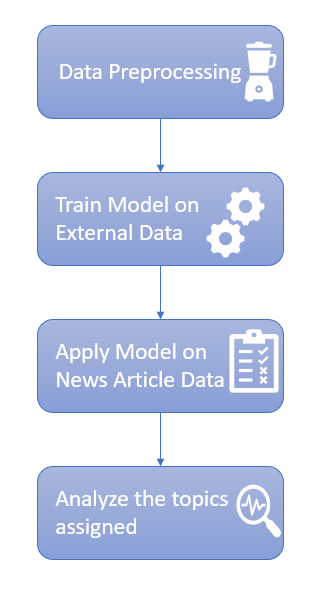
\includegraphics[scale=1]{lda_eda_process.PNG}

\caption{Workflow}
\end{figure}



For data prepossessing we use the steps including:
\begin{itemize}
	\item Removal of special characters
	\item Removal of stop words
    \item Making Bigrams 
    \item Lemmatization
\end{itemize}
Our next step was to use this data to model the topics for the external data. We plot the coherence score vs number of topics to help us get the optimum number of topics. 
\begin{figure}[H]
    \centering
    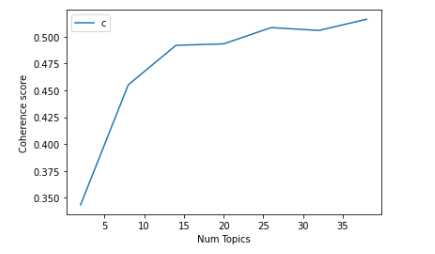
\includegraphics[scale=1.5]{score.PNG}
    \caption{Topic Number vs Coherence Score}
    \label{Topic Number vs Coherence Scorel}
\end{figure}
\\\\

We notice that the optimum number of topics is 15. We create a LDA model with this hyper parameter. We can visualise the topics as well as the words which make up the topic.
\begin{figure}[H]
    \centering
    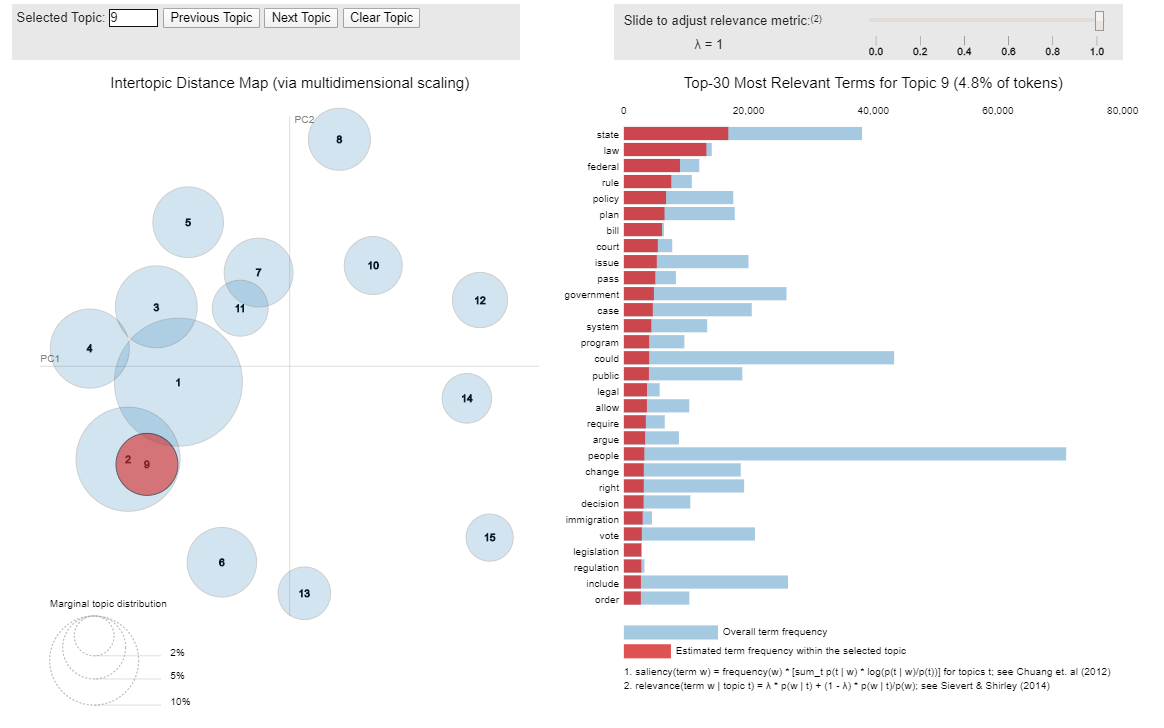
\includegraphics[scale=0.7]{poli.PNG}
    \caption{Visualisation to explore topics and keywords}
    \label{Visualisation to explore topics and keywords}
\end{figure}
\\

Next we apply the model on the dataset of 515 news articles, to get the predominant topics in the dataset. Assigning the topic to with the maximum score to the document and plotting the count of documents for each topic gives the following graph:

\begin{figure}[H]
    \centering
    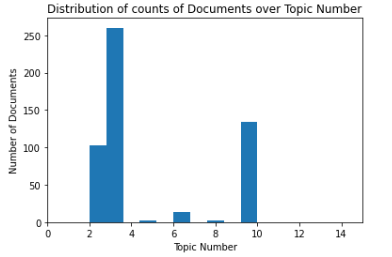
\includegraphics[scale=1]{dist.PNG}
    \caption{Topic number vs Count of documents in news articles data}
    \label{Topic number vs Count of documents in news articles data}
\end{figure}
\\ 

\\Thus we see that only 3 of the topics are pre-dominant in our document. By analysis of the keywords we see all three of these topics are related to politics. Also we observe that 2 and 9 are the topic numbers which are most  frequently occurring, which is consistent with Figure \ref{Visualisation to explore topics and keywords}. 

Also, we use k-means to find the distribution of the topics in the news articles data. First to find the optimum number of clusters in the data, we plot a SSE and number of clusters plot. We get the following graph:
\begin{figure}[H]
    \centering
    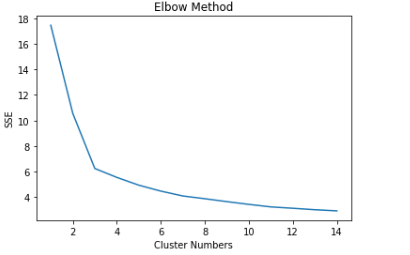
\includegraphics{sse.PNG}
    \caption{Number of clusters vs SSE}
    \label{Number of clusters vs SSE}
\end{figure}

We find that the number of clusters is 3 and this is consistent with the find from figure \ref{Topic number vs Count of documents in news articles data}. The distribution of documents for among the cluster  is:
\begin{figure}[H]
    \centering
    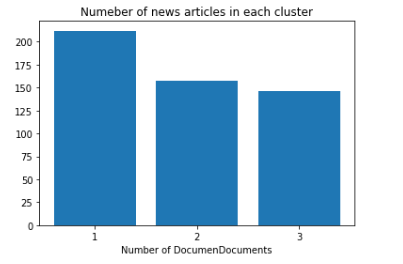
\includegraphics{cluster.PNG}
    \caption{Number of Documents in each cluster}
    \label{Number of Documents in each cluster}
\end{figure}



Thus, we conclude that we need to further divide the topics into sub-topics for analysis.


\section{Algorithm}

\begin{figure}[H]
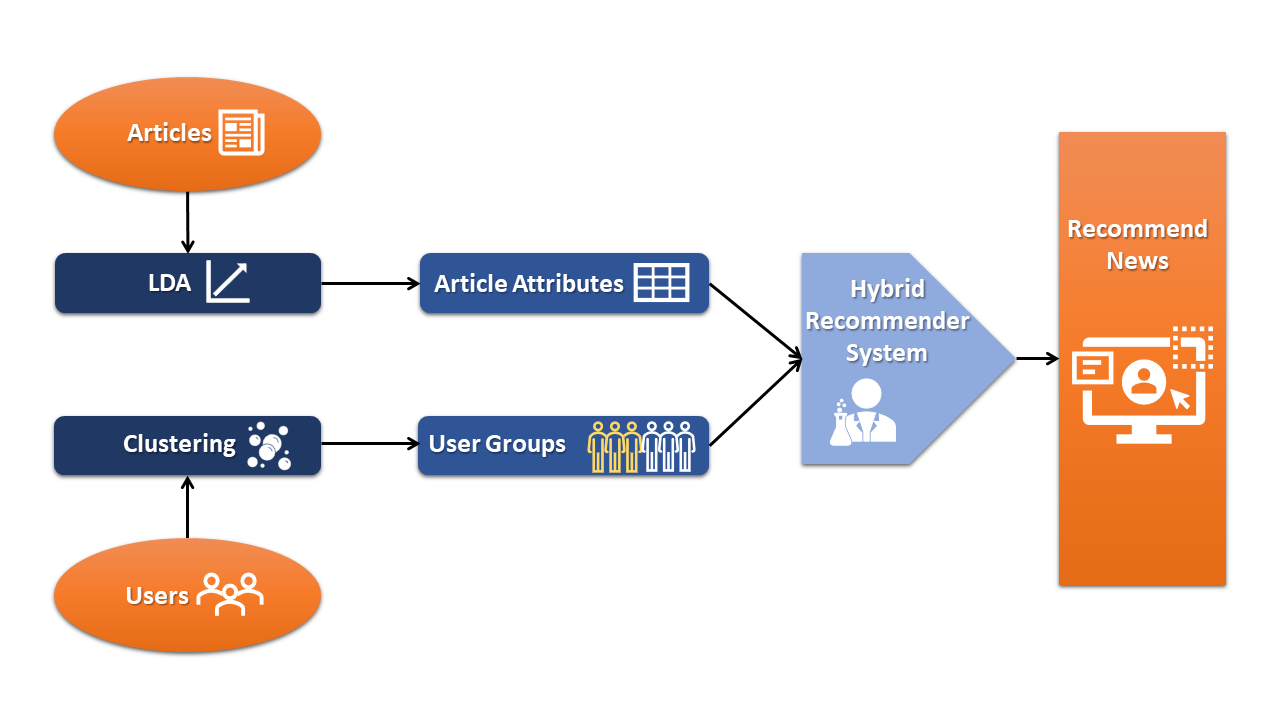
\includegraphics[scale=.40]{NeuRIPS2019/Slide1.PNG}
\caption{Workflow}
\end{figure}

\subsection{Article profiling using LDA}

\subsection{User profiling using Clustering}

\subsection{Hybrid CF-CBF Algorithm for News Recommendation}

\section{Conclusion}

{Description of general difficulties with your problem which bear elaboration
}

\begin{thebibliography}{9}

\bibitem{litReview} Çano, E.,\& Morisio, M.\ (2017). Hybrid recommender systems: A systematic literature review. {\it Intelligent Data Analysis}, 21(6), 1487-1524.
\end{thebibliography}
\end{document}
